
\begin{multicols*}{3}
    \subsection{Tabelle mit Ableitungen und Stammfunktionen}

    \begin{center}
        \renewcommand{\arraystretch}{1.75}
        \begin{tabular} {r c c c l} \toprule
            $f'(x)$                               & \hspace*{-10pt}
            $\xleftrightharpoons[\int f(x) dx]{\frac{d}{dx}}$
            \hspace*{-10pt}                       & $f(x)$          & \hspace*{-10pt}
            $\xleftrightharpoons[\int f(x) dx]{\frac{d}{dx}}$
            \hspace*{-10pt}                       & $F(x)$                                                                                \\
            \midrule
            $n \cdot x^{n - 1}$                   & \hspace*{-20pt} & $x^n$              & \hspace*{-20pt} & $\dfrac{1}{n + 1} x^{n + 1}$ \\
            $e^x$                                 & \hspace*{-20pt} & $e^x$              & \hspace*{-20pt} & $e^x$                        \\
            $\dfrac{1}{x}$                        & \hspace*{-20pt} & $\log|x|$          & \hspace*{-20pt} & $x (\log|x| - 1)$            \\
            \midrule
            $\cos(x)$                             & \hspace*{-20pt} & $\sin(x)$          & \hspace*{-20pt} & $-\cos(x)$                   \\
            $-\sin(x)$                            & \hspace*{-20pt} & $\cos(x)$          & \hspace*{-20pt} & $\sin(x)$                    \\
            $\frac{1}{\cos^2(x)} = 1 + \tan^2(x)$ & \hspace*{-20pt} & $\tan(x)$          & \hspace*{-20pt} & $-\log|\cos(x)|$             \\
            \midrule
            $\dfrac{1}{\log(a) \cdot x}$          & \hspace*{-20pt} & $\log_a|x|$        & \hspace*{-20pt} &                              \\
            $\log(a) \cdot a^x$                   & \hspace*{-20pt} & $a^x$              & \hspace*{-20pt} & $\dfrac{1}{\log(a)} a^x$     \\
            $x^x (\log(x)+1)$                     & \hspace*{-20pt} & $x^x$              & \hspace*{-20pt} &                              \\
            \midrule
            $\cosh(x)$                            & \hspace*{-20pt} & $\sinh(x)$         & \hspace*{-20pt} &                              \\
            $\sinh(x)$                            & \hspace*{-20pt} & $\cosh(x)$         & \hspace*{-20pt} &                              \\
            $\dfrac{1}{\cosh^2(x)}$               & \hspace*{-20pt} & $\tanh(x)$         & \hspace*{-20pt} & $\log(\cosh(x))$             \\
            \midrule
            $\dfrac{1}{\sqrt{1 - x^2}}$           & \hspace*{-20pt} & $\arcsin(x)$       & \hspace*{-20pt} &                              \\
            $- \dfrac{1}{\sqrt{1 - x^2}}$         & \hspace*{-20pt} & $\arccos(x)$       & \hspace*{-20pt} &                              \\
            $\dfrac{1}{1 + x^2}$                  & \hspace*{-20pt} & $\arctan(x)$       & \hspace*{-20pt} &                              \\
            \midrule
            $\dfrac{1}{\sqrt[]{x^2 + 1}}$         & \hspace*{-20pt} & $\text{arsinh}(x)$ & \hspace*{-20pt} &                              \\
            $\dfrac{1}{\sqrt[]{x^2 - 1}}$         & \hspace*{-20pt} & $\text{arcosh}(x)$ & \hspace*{-20pt} &                              \\
            $\dfrac{1}{1 - x^2}$                  & \hspace*{-20pt} & $\text{artanh}(x)$ & \hspace*{-20pt} &                              \\
            \midrule
            $\text{sign}(x) = \begin{cases}
                                      -1 & x < 0 \\  1 & 0 < x \\
                                  \end{cases}$ \hspace*{-10pt}       & \hspace*{-20pt} & $|x|$              & \hspace*{-20pt} &               \\
            \bottomrule
        \end{tabular}
    \end{center}

    Bemerkung: Bei Ableitungen mit Logarithmen, sowie den inversen Trigo- und Hyperfunktionen ist der Definitionsbereich eingeschränkt!


    \subsection{Stetige Funktionen}

    Folgende Elementarfunktionen sind stetig auf ihrem Definitionsbereich:

    \begin{center}
        \begin{tabular}{l} \toprule
            i) Polynome sind stetige Funktionen auf $\R$.                                                 \\
            ii) Rationale Funktionen $\frac{p}{q}$ sind stetig auf $\Omega = \{ z \in \C; q(z) \neq 0\}$. \\
            iii) Die Wurzelfunktion ist auf $\R_+$ stetig.                                                \\
            iv) Die Exponentialfunktion ist auf $\R$ stetig.                                              \\
            v) Die Logartihmusfunktion ist auf $]0, \infty[$ stetig.                                      \\
            \bottomrule
        \end{tabular}
    \end{center}
    \vfill\null
    \columnbreak


    \subsection{Partialbruchzerlegung}

    Ziel: Rationale Funktionen $\left(\frac{p(x)}{q(x)}\right)$ in Teilbrüche zerlegen. Vorgehen: \medskip

    i) Wenn der Zähler einen höheren Grad als den Nenner hat, muss man zuerst eine Polynomdivision durchführen, d.h. $\left(p(x):q(x) = \dots\right)$. \medskip

    ii) Das Nennerpolynom $q(x)$ in Nullstellenform bringen.

    \begin{center}
        $q(x) = \prod\limits_{i = 1} (x - x_i)^{m_i}$ \qquad wobei $(x - x_i) = 0$
    \end{center}

    iii) a) Die Nullstelle hat Multiplizität 1 ($m_i = 1$):

    \begin{center}
        $\dfrac{C}{(x - x_i)}$
    \end{center}

    b) Die Nullstelle hat Multiplizität grösser 1 ($1 < m_i$):

    \begin{center}
        $\dfrac{C_1}{(x - x_i)} + \dfrac{C_2}{(x - x_i)^2} + \dots + \dfrac{C_{m_i}}{(x - x_i)^{m_i}}$
    \end{center}

    c) Die Nullstelle ist komplexwertig (Gewünschte Form: $ax^2 + b x + c$):

    \begin{center}
        $\dfrac{Ax + B}{(a x^2 + b x + c)}$
    \end{center}

    iii) Alle Koeffizienten $C_i$ bestimmen durch einen Koeffizientenvergleich.
    \vfill\null
    \columnbreak


    \section{Ergänzungen aus LinAlg}

    \subsection{Determinante}

    Sei $A \in M_{2 \times 2}(\R)$. Dann ist die Determinante:

    \begin{center}
        \eqbox{$\det\begin{bmatrix}
                    a & b \\ c & d \\
                \end{bmatrix} := a d - b c$}
    \end{center}


    \subsubsection{Laplace Entwicklung}

    Sei die Matrix $A = \begin{bmatrix}
            a_1 & b_1 & c_1 \\ a_2 & b_2 & c_2 \\ a_3 & b_3 & c_3 \\
        \end{bmatrix}$. Die Entwicklung nach Zeile 2 ist:

    \begin{center}
        $\det(A) = -a_2 \cdot \det\begin{bmatrix}
                b_1 & c_1 \\ b_3 & c_3 \\
            \end{bmatrix} + b_2 \cdot \det\begin{bmatrix}
                a_1 & c_1 \\ a_3 & c_3 \\
            \end{bmatrix} - c_2 \cdot \det \begin{bmatrix}
                a_1 & b_1 \\ a_3 & b_3 \\
            \end{bmatrix}$
    \end{center}

    Für die Vorzeichen gilt zu beachten: $\begin{bmatrix}
            + & - & + & - \\
            - & + & - & + \\
            + & - & + & - \\
            - & + & - & + \\
        \end{bmatrix}$


    \subsection{Eigenwerte und Eigenvektoren}

    Die Eigenwerte einer Matrix $A$ berechnet man mit

    \begin{center}
        \eqbox{$\det(A - \lambda I) = 0$}
    \end{center}

    Der zum Eigenwert $\lambda_i$ dazugehörige Eigenvektor $\vect{s}_i$ berechnet man durch das Auflösen von folgendem homogenen LGS:

    \begin{center}
        \eqbox{$(A - \lambda_i I) \cdot \vect{s}_i = \vect{0}$}
    \end{center}


    \subsubsection{Diagonalisierbar}

    Sei $A \in M_{n \times n}(\R)$ mit $n$ linear unabhängigen Eigenvektoren $\vect{s}_1$ und seien $\lambda_1, \dots, \lambda_n$ die Eigenwerte von $A$. Dann ist $A$ diagonalisierbar:

    \begin{center}
        \eqbox{$A = S D S^{-1} = [\vect{s}_1 \dots \vect{s}_n] \begin{bmatrix}
                \lambda_1 &        & 0         \\
                          & \ddots &           \\
                0         &        & \lambda_n \\
            \end{bmatrix} [\vect{s}_1 \dots \vect{s}_n]^{-1}$}
    \end{center}


    \subsection{Matrixinverse berechen}

    Zuerst Gauss-Elimination, dann Rücksubstitution ($[A | I] \Rightarrow [I | A^{-1}]$)

    \subsubsection{Explizite Formeln}

    Für $A \in M_{2 \times 2}(\R)$ gilt:

    \begin{center}
        \eqbox{$A^{-1} = \begin{bmatrix}
                a & b \\
                c & d \\
            \end{bmatrix}^{-1} = \dfrac{1}{\det(A)} \cdot
            \begin{bmatrix}
                d  & -b \\
                -c & a  \\
            \end{bmatrix}$}
    \end{center}

    Für $A \in M_{3 \times 3}(\R)$ gilt:

    \begin{center}
        $A^{-1} = \begin{bmatrix}
                a & b & c \\
                d & e & f \\
                g & h & i \\
            \end{bmatrix}^{-1} = \dfrac{1}{\det(A)} \cdot
            \begin{bmatrix}
                ei - fh & ch - bi & bf - ce \\
                fg - di & ai - cg & cd - af \\
                dh - eg & bg - ah & ae - bd \\
            \end{bmatrix}$
    \end{center}
\end{multicols*}


\begin{multicols*}{2}
    \section{Spass mit Integralen}

    \subsection{Tangenssubstitution}

    Sei $t(x) = \tan(\frac{x}{2})$ mit $x \in ]-\pi, \pi[$. Dann gilt

    \begin{center}
        \renewcommand{\arraystretch}{1.5}
        \begin{tabular}{l l} \toprule
            $\cos(x) = \dfrac{1 - t^2(x)}{1 + t^2(x)}$ & $\sin(x) = \dfrac{2 t(x)}{1 + t^2(x)}$   \\
            $\cos^2(x) = \dfrac{1}{1 + t^2(x)}$        & $\sin^2(x) = \dfrac{t^2(x)}{1 + t^2(x)}$ \\
            \bottomrule
        \end{tabular}
    \end{center}

    Mit dieser Substitution kann man gewisse Trigonometrische Integrale einfacher lösen.
    \subsection{Rückwärtssubstitution}

    Die Substitutionsregel lässt sich auch rückwärts durchführen. Sei $\varphi(x)$ \emph{injektiv}. Dann gilt:

    \begin{center}
        \eqboxf{$\displaystyle \int\limits_{\alpha}^{\beta} f(t) dt = \int\limits_{\varphi^{-1}(\alpha)}^{\varphi^{-1}(\beta)} f\left( \varphi(x) \right) \cdot \varphi'(x) dx$}
    \end{center}

    Bei geschickter Wahl der Funktion $\varphi(x)$ kann entgegen des ersten Anscheins der Integrand vereinfacht werden.

    \subsubsection{Tabelle}
    %https://de.wikipedia.org/wiki/Integration_durch_Substitution#Anwendung
    %https://en.wikipedia.org/wiki/Trigonometric_substitution

    Bem: Nach Anwendung der Regel ist die Trigo-Identiät ($cos^2(x) + sin^2(x) = 1$) notwendig!

    \begin{center}
        \renewcommand{\arraystretch}{2}
        \begin{tabular}{c l l l} \toprule
            \textbf{Integral}                                             & \multicolumn{2}{l}{\textbf{Rücksubstitution}}                                                                                          \\
            \midrule 
            $\int\limits_{\alpha}^{\beta} \sqrt{1 - t^2} dt$              & $\varphi(x) = \sin(x)$                        & $\varphi^{-1}(t) = \arcsin(t)$                       & $\varphi'(x) = \cos(x)$         \\
            \midrule
            $\int\limits_{\alpha}^{\beta} \sqrt{a^2 - t^2} dt$            & $\varphi(x) = a \cdot \sin(x)$                & $\varphi^{-1}(t) = \arcsin\left(\dfrac{t}{a}\right)$ & $\varphi'(x) = a \cdot \cos(x)$ \\
            $\int\limits_{\alpha}^{\beta} \dfrac{1}{\sqrt{a^2 - t^2}} dt$ & $\varphi(x) = a \cdot \sin(x)$                & $\varphi^{-1}(t) = \arcsin\left(\dfrac{t}{a}\right)$ & $\varphi'(x) = a \cdot \cos(x)$ \\
            \midrule
            $\int\limits_{\alpha}^{\beta} \sqrt{1 + t^2} dt$              & $\varphi(x) = \sinh(x)$                       & $\varphi^{-1}(t) = \text{arsinh}(t)$                 & $\varphi'(x) = \cosh(x)$        \\
            $\int\limits_{\alpha}^{\beta} \sqrt{t^2 - 1} dt$              & $\varphi(x) = \cosh(x)$                       & $\varphi^{-1}(t) = \text{arcosh}(t)$                 & $\varphi'(x) = \sinh(x)$        \\
            \bottomrule
        \end{tabular}
    \end{center}


    \subsection{Integrale über eine Periode (Orthogonalitätsrelationen)}

    Sei $\omega = \dfrac{2\pi}{T}$ und $m,n \in \N$. Dann gelten folgende Relationen:

    \begin{center}
        \begin{tabular}{l c l} \toprule
            $\displaystyle\int\limits_0^T \sin(n \omega t) dt = 0$                             & \hspace*{+20pt} &
            $\displaystyle\int\limits_0^T \cos(n \omega t) dt = 0$                                                                                                                                                         \\
            \midrule
            $\displaystyle\int\limits_0^T \sin(n \omega t) \sin(m \omega t) dt = \begin{cases}
                                                                                         0 & n \neq m \\ \frac{T}{2} & n = m \\
                                                                                     \end{cases}$ & \hspace*{+20pt} & $\displaystyle\int\limits_0^T \cos(n \omega t) \cos(m \omega t) dt = \begin{cases}
                                                                                                                                                                                               0 & n \neq m \\ \frac{T}{2} & n = m \\
                                                                                                                                                                                           \end{cases}$ \\
            \midrule
            $\displaystyle\int\limits_0^T \sin(n \omega t) \cos(m \omega t) dt = 0$                                                                                                                                        \\
            \toprule
        \end{tabular}
    \end{center}
    \vfill\null
    \columnbreak

    \subsection{Liste von Trigonometrischen Integralen}

    Man kann diese Integrale \emph{normalerweise} benutzen bei der Prüfung, solange man auf die Identität vermerkt. Man setzt dabei einfach die Integralgrenzen ein, wie man es intuitiv machen würde.

    \begin{center}
        \renewcommand{\arraystretch}{1.5}
        \begin{tabular}{l c l} \toprule
            $\displaystyle \int \sin^2(x) dx = \dfrac{x - \sin(x)\cos(x)}{2} + C$                                    & \hspace*{+10pt} & $\displaystyle \int\frac{1}{\sin{(x)}}dx =\ln{\vert\frac{\sin{(x)}}{\cos{(x)}+1}\vert} + C$             \\
            $\displaystyle \int \cos^2(x) dx = \dfrac{x + \sin(x)\cos(x)}{2} + C$                                    & \hspace*{+10pt} & $\displaystyle \int\frac{1}{\cos{(x)}}dx =\ln{\vert\frac{-\cos{(x)}}{\sin{(x)}-1}\vert} + C$            \\
            $\displaystyle \int \sin(x) \cos(x) dx = \dfrac{sin^2(x)}{2} + C$                                        & \hspace*{+10pt} & $\displaystyle \int \frac{1}{\tan(x)} dx =\ln\vert \sin(x) \vert + C$                                   \\
            $\displaystyle \int \sin^2(x)\cos(x)dx = \frac{1}{3}\sin^3(x) + C$                                       & \hspace*{+10pt} & $\displaystyle \int \frac{1}{\cos^2(x)}dx =\tan(x) + C$                                                 \\
            $\displaystyle \int \sin(x)\cos^2(x)dx = -\frac{1}{3}\cos^3(x) + C$                                      & \hspace*{+10pt} & $\displaystyle \int \frac{1}{\sin^2{(x)}}dx =-\frac{1}{\tan{(x)}} + C$                                  \\
            $\displaystyle \int \sin^2(x)\cos^2(x)dx = \frac{1}{32}(4x-\sin(4x)) + C$                                & \hspace*{+10pt} & $\displaystyle \int \arcsin(x)dx = x\cdot \arcsin(x)+\sqrt{1-x^2} + C$                                  \\
            $\displaystyle \int \arccos(x)dx =x\cdot \arccos(x)-\sqrt{1-x^2} + C$                                    & \hspace*{+10pt} & $\displaystyle \int \arctan(x)dx =x\cdot \arctan(x)-\frac{1}{2}\ln \vert x^2+1\vert + C$                \\
            \midrule
            $\displaystyle \int_0^{2\pi}\cos^4(t)\text{dt} =\displaystyle \int_0^{2\pi}\sin^4(t)dt = \frac{3\pi}{4}$ & \hspace*{+10pt} & $\displaystyle \int_0^{2\pi}\cos^3(t)\text{dt} =\displaystyle \int_0^{2\pi}\sin^3(t)dt = 0$             \\
            $\displaystyle \int_0^{2\pi}\cos^2(t)\text{dt} =\displaystyle \int_0^{2\pi}\sin^2(t)dt = \pi$            & \hspace*{+10pt} & $\displaystyle \int_0^{2\pi}\sin(t)\cos^2(t)\text{dt} =\displaystyle \int_0^{2\pi}\cos(t)\sin^2(t)dt=0$ \\
            $\displaystyle \int_0^{2\pi}\sin(t)\cos(t)\text{dt} =0$                                                  & \hspace*{+10pt} &                                                                                                         \\
            \toprule
        \end{tabular}
    \end{center}

    \subsubsection{Tabelle von ausgewerteten Integralen}

    Mit der Begründung ''Symmetrie'' ist es normalerweise erlaubt die \emph{Nullintegrale} der Tabelle zu benutzen. \medskip

    Den Rest der Tabelle würde ich nur zur Überprüfung der Resultate an der Prüfung verwenden. Denke nicht, dass es Pünkte gibt, wenn man direkt das Resultat schreibt.

    \begin{center}
        \renewcommand{\arraystretch}{1.5}
        \begin{tabular}{ r c c c c c c c }\toprule
            \textbf{Funktion:}     & \multicolumn{5}{l}{\textbf{Integralgrenzen:}}                                                                                                                                                                                                                                                       \\
            \midrule
                                   & $\displaystyle\int_0^{\frac{\pi}{4}}$         & $\displaystyle\int_0^{\frac{\pi}{2}}$ & $\displaystyle\int_0^{\pi}$ & $\displaystyle\int_0^{2\pi}$ & $\displaystyle\int_{-\frac{\pi}{4}}^{\frac{\pi}{4}}$ & $\displaystyle\int_{-\frac{\pi}{2}}^{\frac{\pi}{2}}$ & $\displaystyle\int_{-\pi}^{\pi}$ \\
            \midrule
            $\sin(x)$              & $\frac{\sqrt{2}-1}{\sqrt{2}}$                 & $1$                                   & $2$                         & $0$                          & $0$                                                  & $0$                                                  & $0$                              \\

            $\sin^2(x)$            & $\frac{\pi-2}{8}$                             & $\frac{\pi}{4}$                       & $\frac{\pi}{2}$             & $\pi$                        & $\frac{\pi-2}{4}$                                    & $\frac{\pi}{2}$                                      & $\pi$                            \\

            $\sin^3(x)$            & $\frac{8-5\sqrt{2}}{12}$                      & $\frac{2}{3}$                         & $\frac{4}{3}$               & $0$                          & $0$                                                  & $0$                                                  & $0$                              \\

            $\cos(x)$              & $\frac{1}{\sqrt{2}}$                          & $1$                                   & $0$                         & $0$                          & $\sqrt{2}$                                           & $2$                                                  & $0$                              \\

            $\cos^2(x)$            & $\frac{2+\pi}{8}$                             & $\frac{\pi}{4}$                       & $\frac{\pi}{2}$             & $\pi$                        & $\frac{2+\pi}{4}$                                    & $\frac{\pi}{2}$                                      & $\pi$                            \\

            $\cos^3(x)$            & $\frac{5}{6\sqrt{2}}$                         & $\frac{2}{3}$                         & $0$                         & $0$                          & $\frac{5}{3\sqrt{2}}$                                & $\frac{4}{3}$                                        & $0$                              \\

            $\sin \cdot \cos(x)$   & $\frac{1}{4}$                                 & $\frac{1}{2}$                         & $0$                         & $0$                          & $0$                                                  & $0$                                                  & $0$                              \\

            $\sin^2 \cdot \cos(x)$ & $\frac{1}{6\sqrt{2}}$                         & $\frac{1}{3}$                         & $0$                         & $0$                          & $\frac{1}{3\sqrt{2}}$                                & $\frac{2}{3}$                                        & $0$                              \\

            $\sin \cdot \cos^2(x)$ & $\frac{4-\sqrt{2}}{12}$                       & $\frac{1}{3}$                         & $\frac{2}{3}$               & $0$                          & $0$                                                  & $0$                                                  & $0$                              \\
            \bottomrule
        \end{tabular}
    \end{center}
\end{multicols*}

\begin{multicols*}{3}
    \section{Relevante Plots}

    \subsection{Trigonometrische Funktionen}

    \begin{center}
        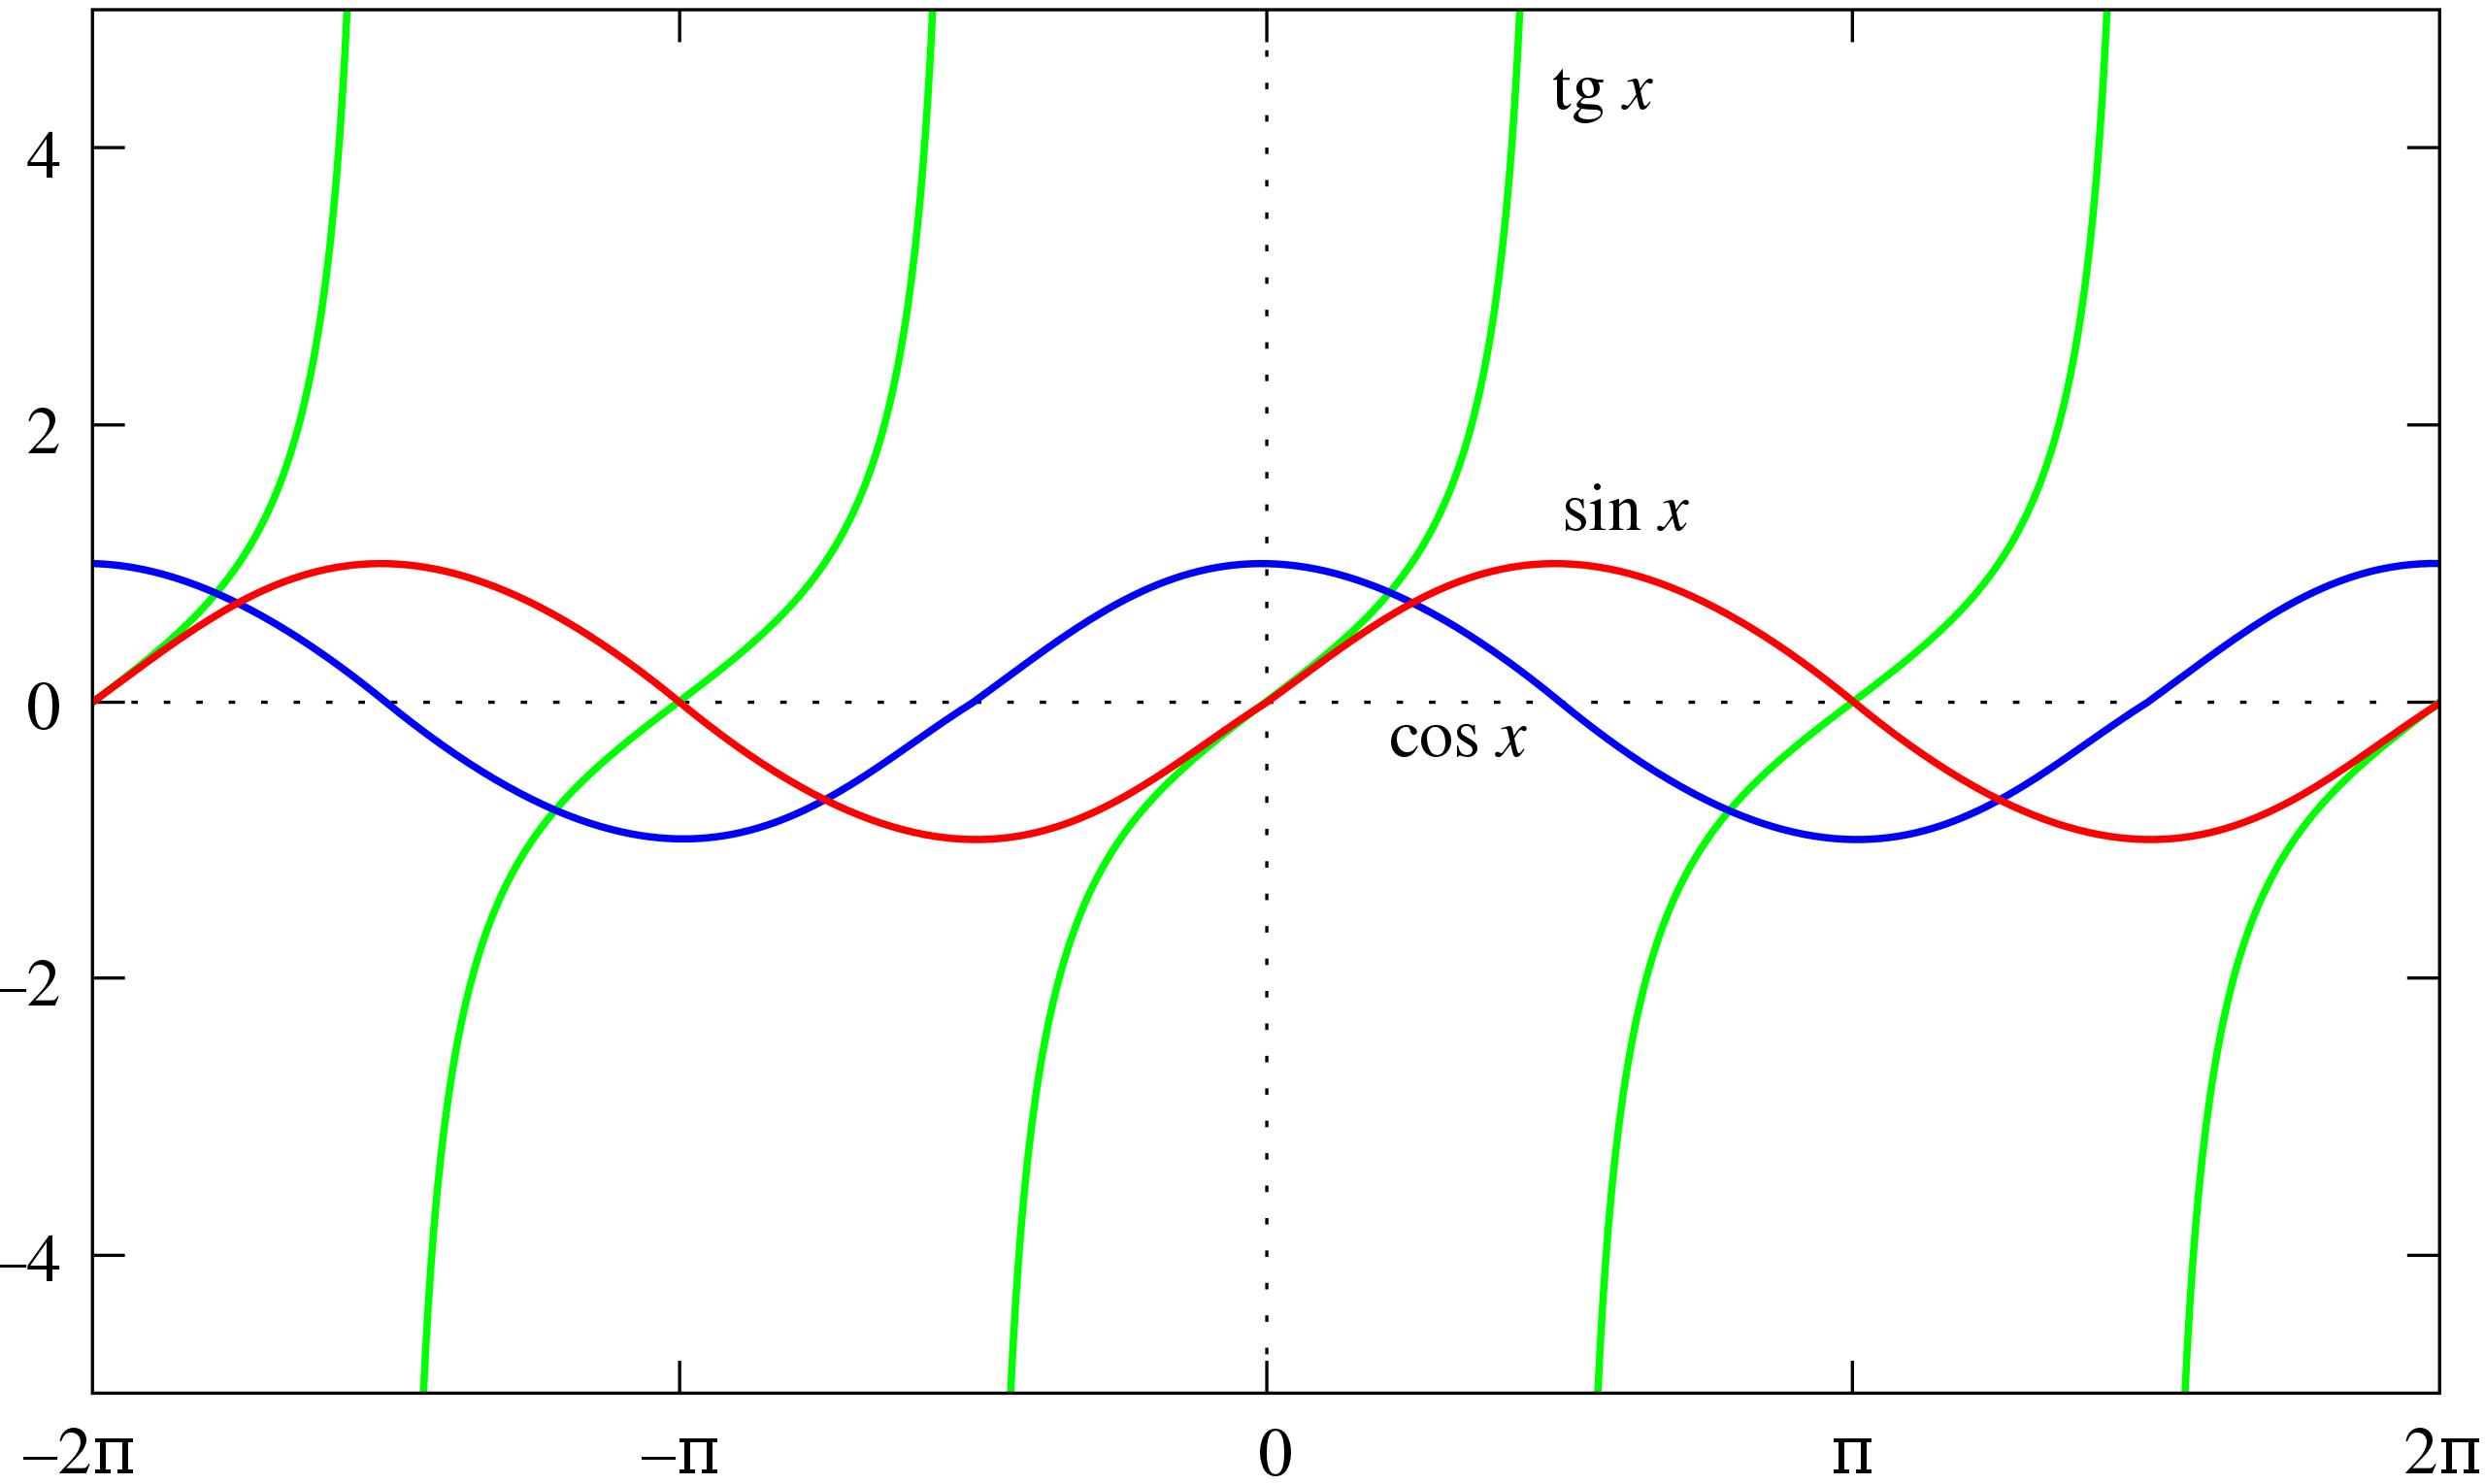
\includegraphics[width=1\linewidth]{Bilder/Trigonometric_functions.png}
    \end{center}

    \subsection{Einheitskreis}

    \begin{center}
        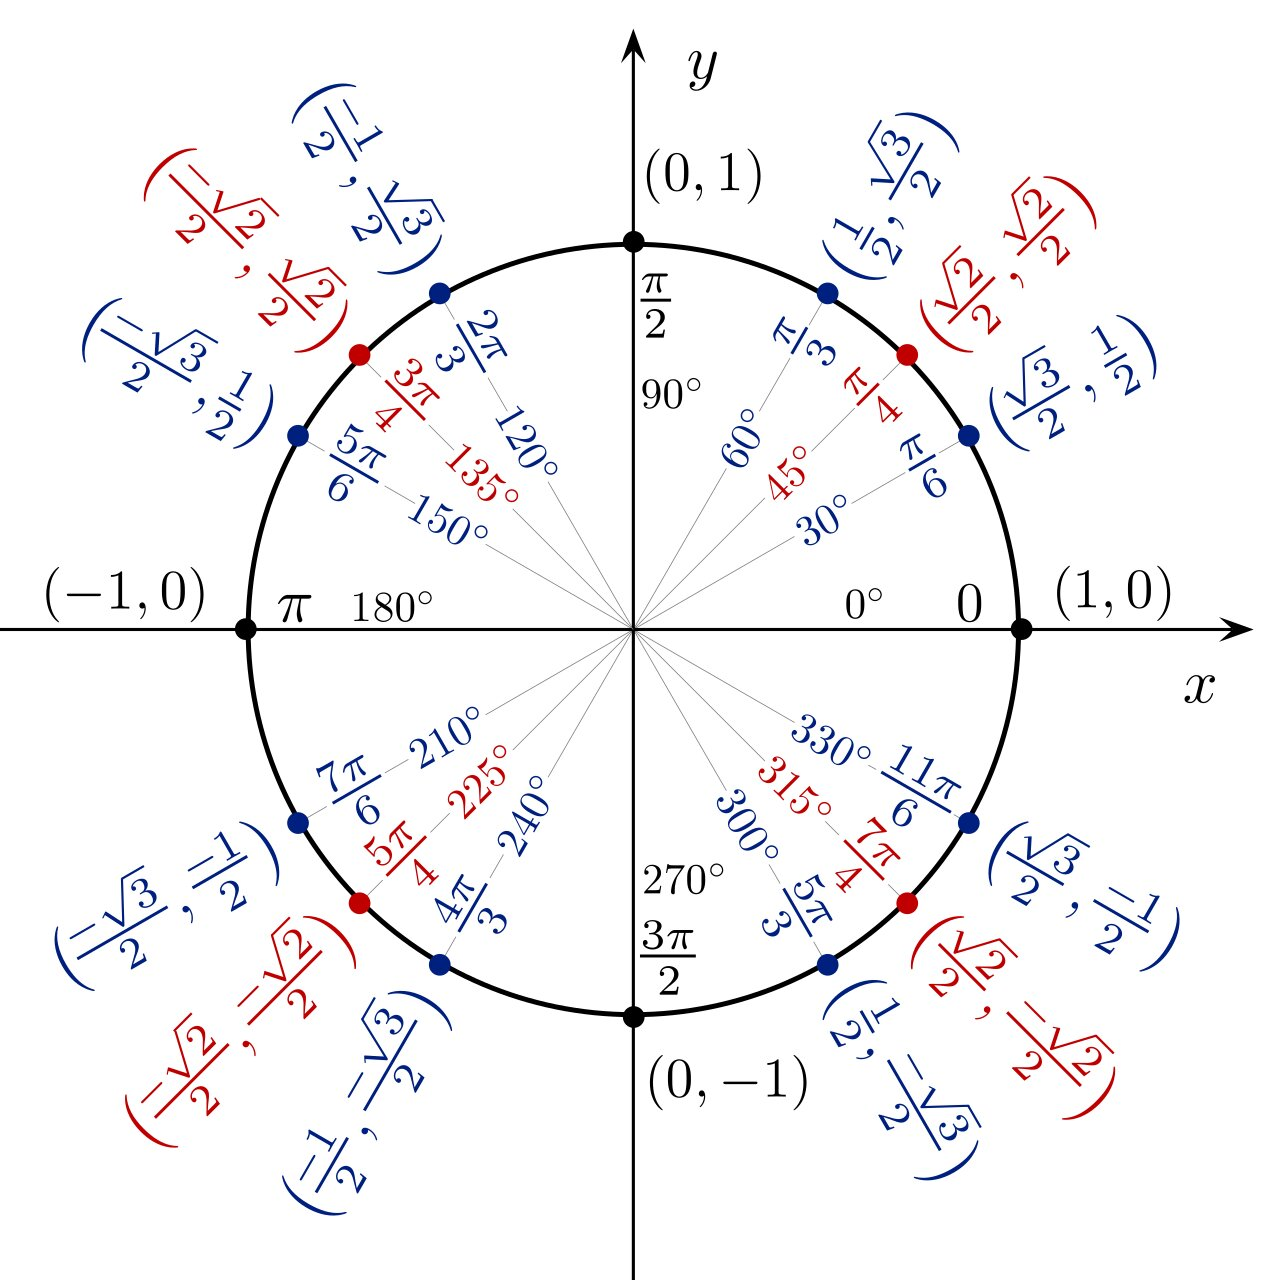
\includegraphics[width=1\linewidth]{Bilder/unit-circle.jpg}
    \end{center}
    \vfill\null
    \columnbreak

    \subsection{Hyperbelfunktionen}

    \begin{center}
        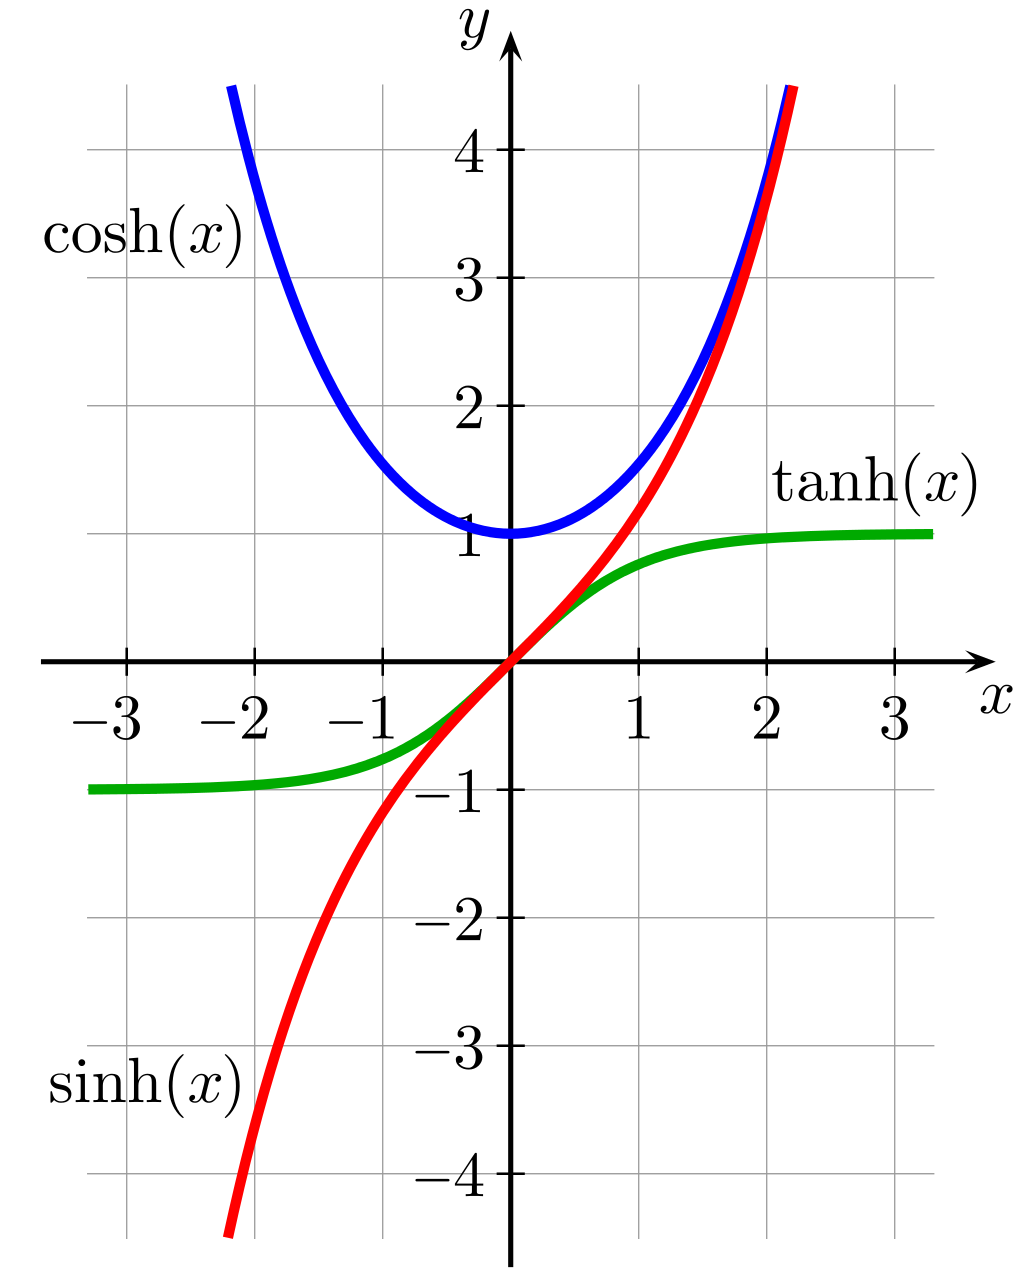
\includegraphics[width=1\linewidth]{Bilder/Sinh_cosh_tanh.png}
    \end{center}
    \vfill\null
    \columnbreak

    \subsection{Areafunktionen (Umkehrfunktionen der Hyperbelfunktionen)}

    \begin{center}
        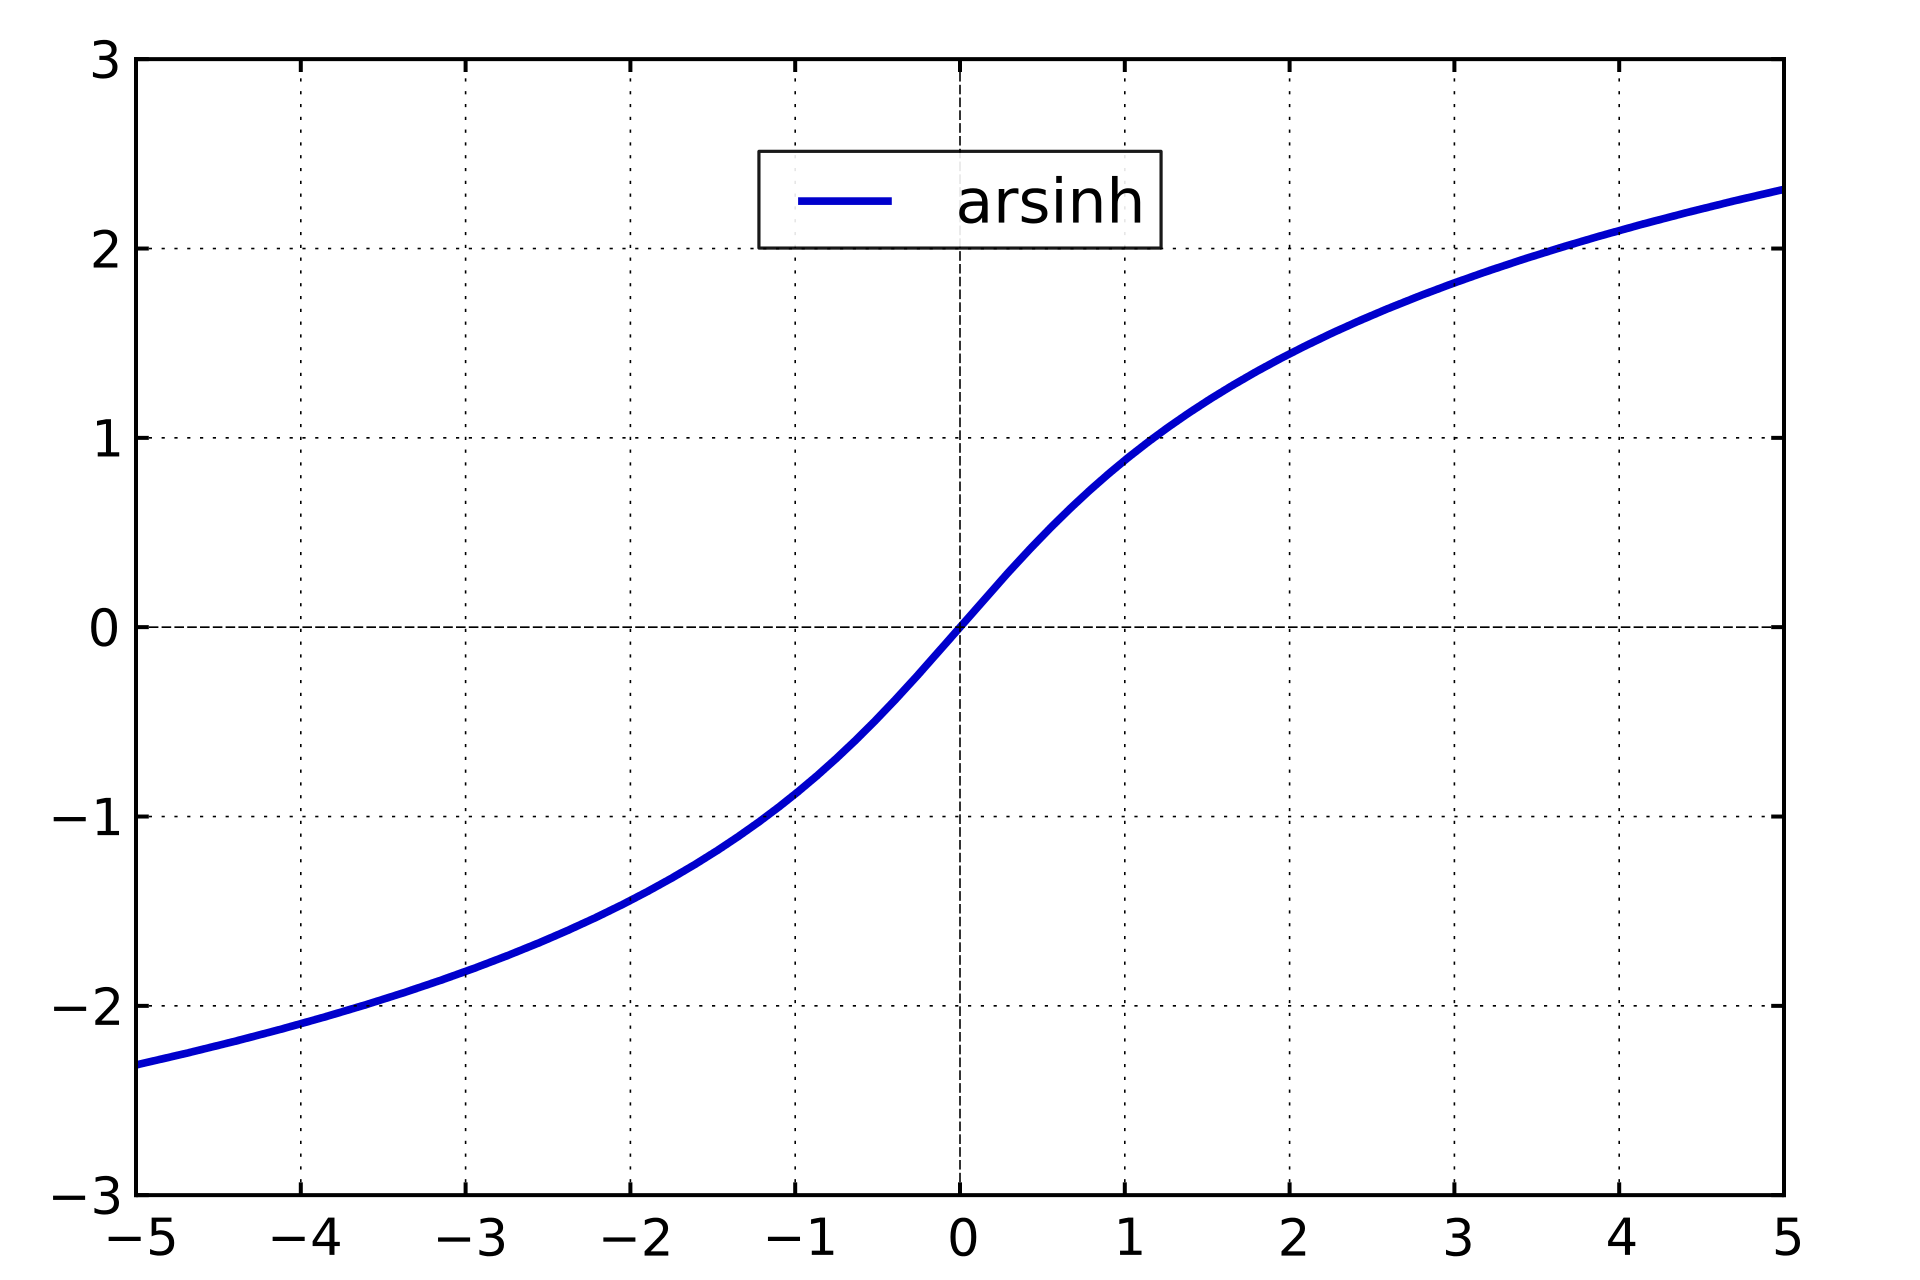
\includegraphics[width=0.95\linewidth]{Bilder/arsinh.png}
    \end{center}

    \begin{center}
        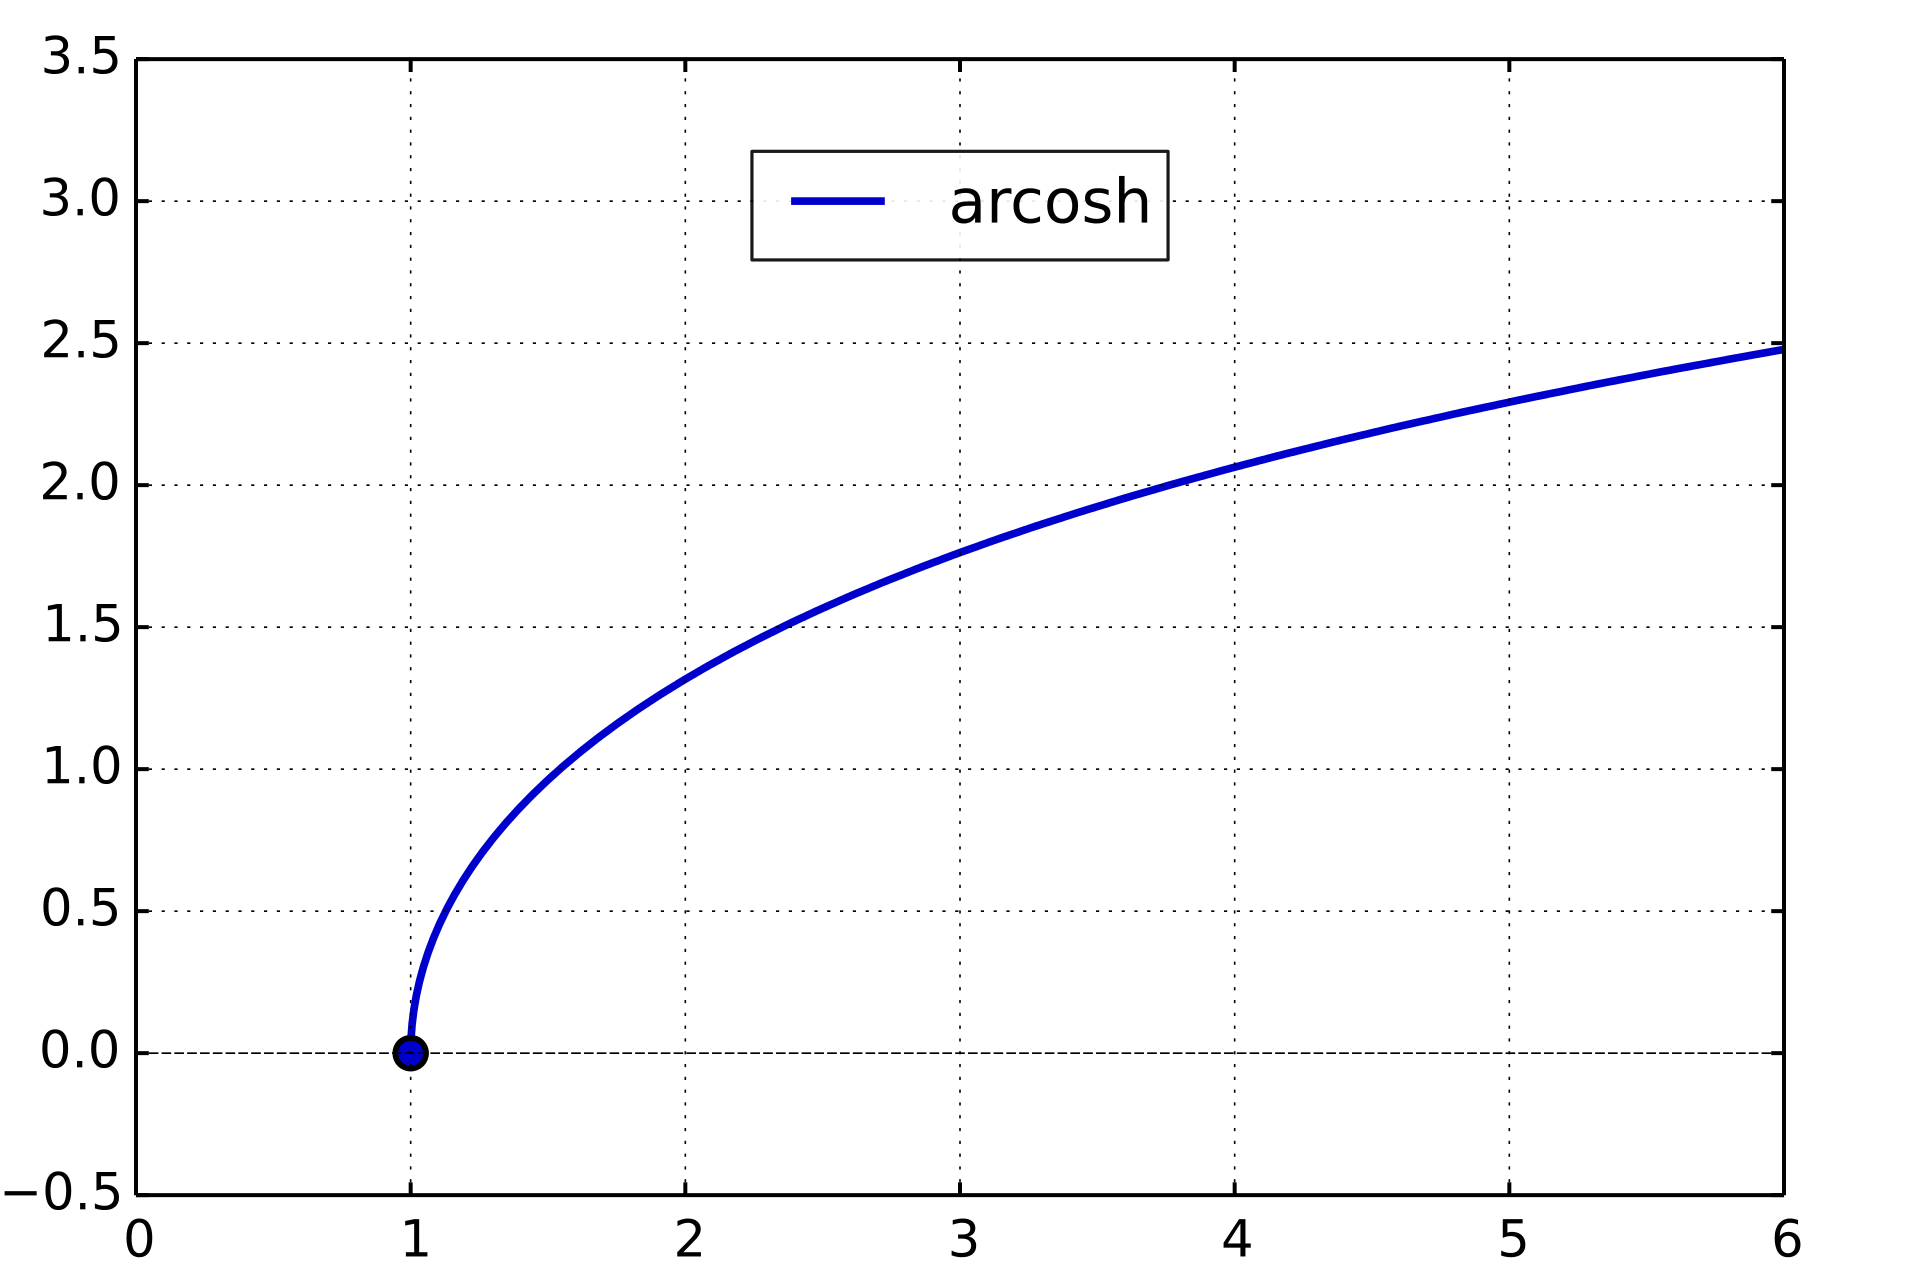
\includegraphics[width=0.95\linewidth]{Bilder/arcosh.png}
    \end{center}

    \begin{center}
        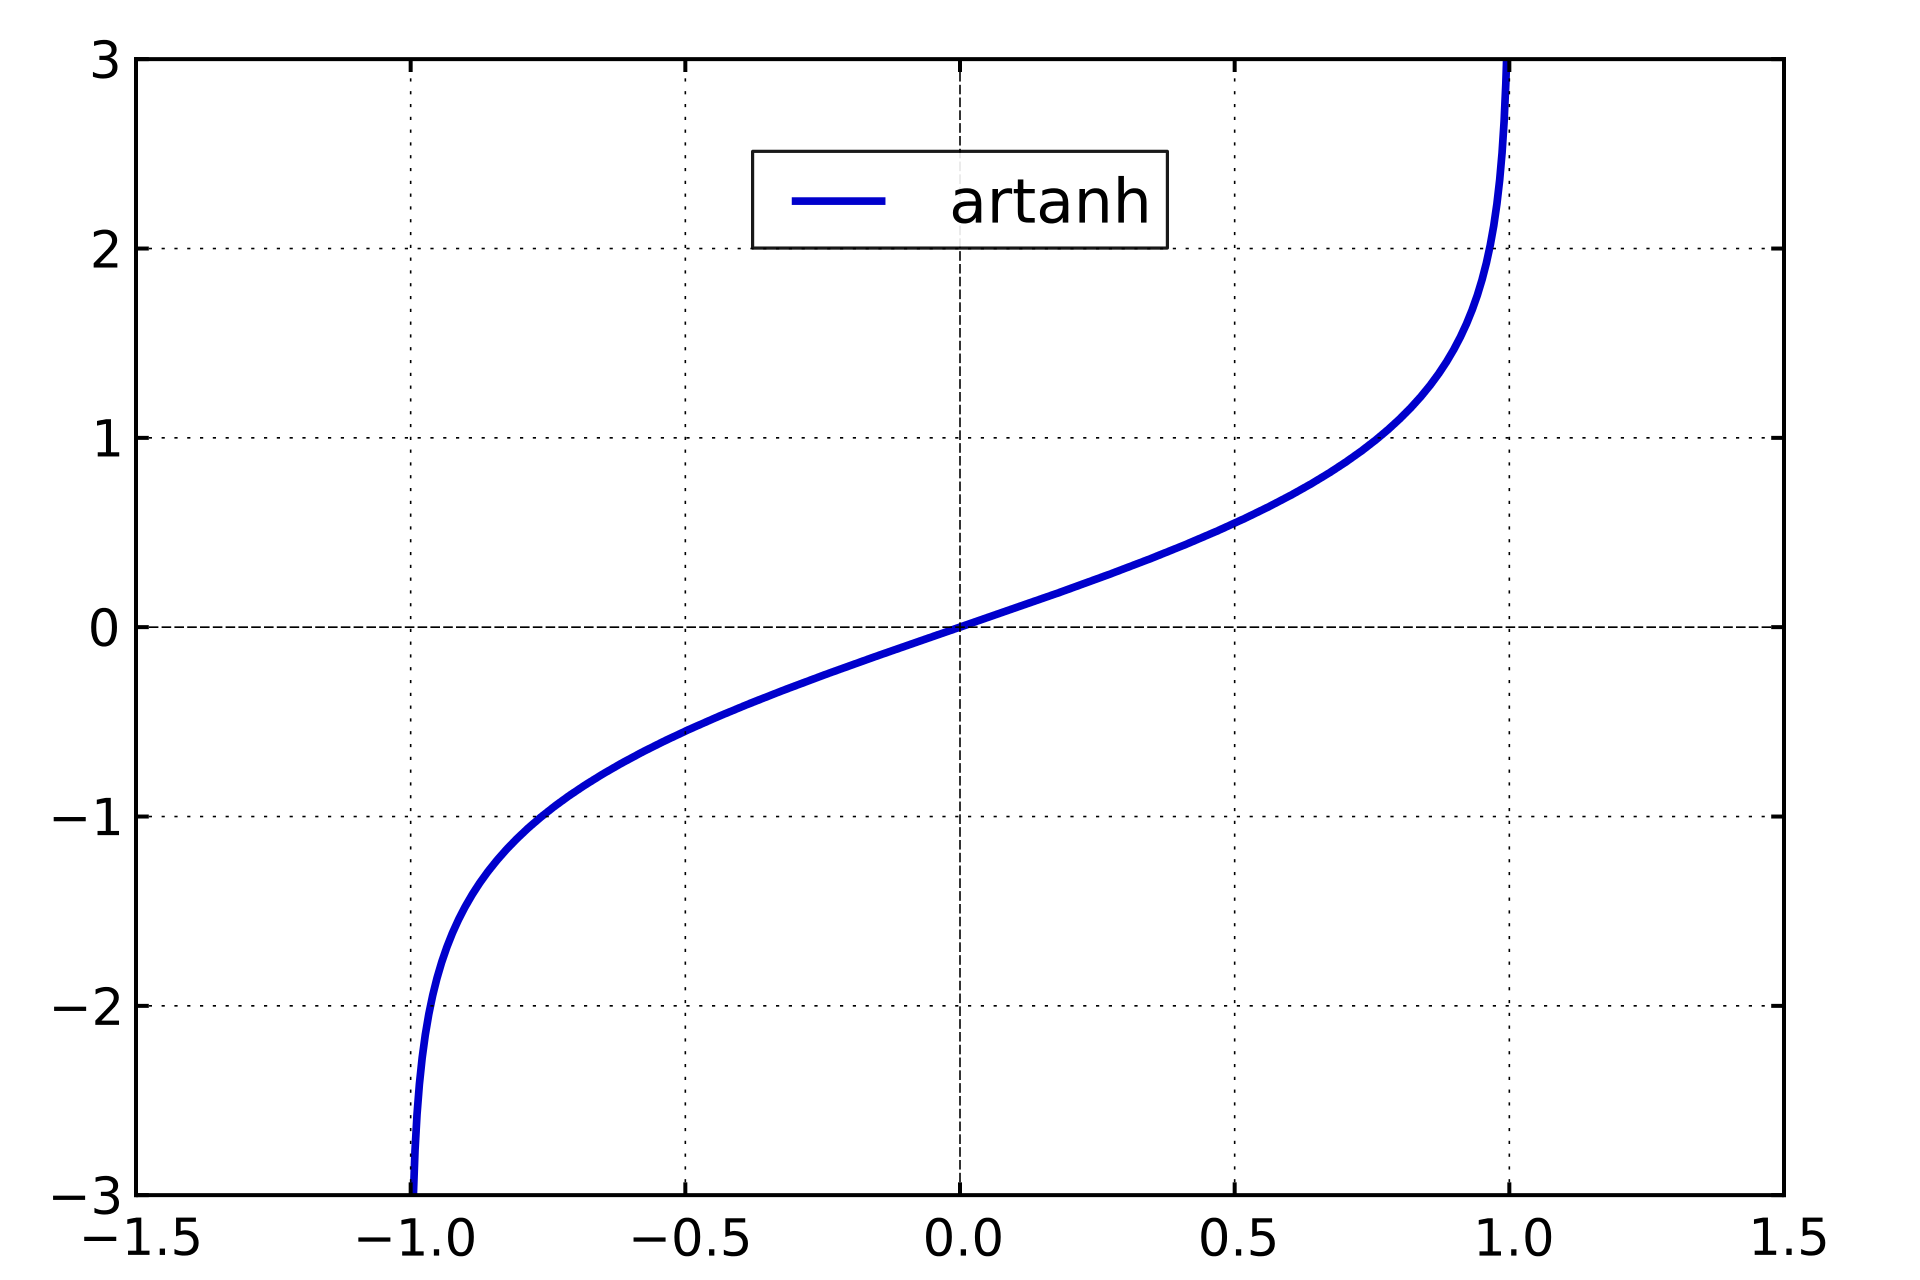
\includegraphics[width=0.95\linewidth]{Bilder/artanh.png}
    \end{center}
\end{multicols*}

\begin{multicols*}{3}
    \subsection{Kochrezepte}

    \subsubsection{Überprüfung auf Differenzierbarkeit}

    Meistens ist der Ursprung $(0,0)$ gefragt mit Funktionen, welche bis auf den Ursprung differenzierbar sind. Das allgemeine Vorgehen ist: \medskip

    i) Auf Stetigkeit überprüfen. \textbf{Polarkoordinantentrick}:

    \begin{center}
        $r^2 = x^2+y^2$ mit $x = r \cdot \cos(\varphi)$ und $y = r \cdot \sin(\varphi)$
    \end{center}
    \medskip

    Falls $\lim\limits_{r \to r_0}$ unabhängig von $\varphi$ existiert, dann ist $f$ stetig in $(x_0,y_0)$. \medskip

    \emph{Unstetigkeit zeigen}: Man untersucht die Grenzwerte verschiedener Folgen $(\frac{1}{n},\frac{1}{n})$ und $(0,\frac{1}{n})$ und zeigt, dass zwei Unterschiedliche Grenzwerte vorhanden sind. \medskip

    ii) Differenzierbarkeit überprüfen: Partielle Ableitungen bestimmen und Definition Differenzierbarkeit einsetzen (evtl. Polarkoordinantentrick für Grenzwert benutzen). \medskip

    \emph{Nicht differenzierbar} zeigen: Neben Unstetigkeit in $(x_0,y_0)$ oder Unstetigkeit von $\partial_x f, \partial_y f$ kann man auch zeigen, dass für $\vec{v} = h\cdot(v_1,v_2)$:

    \begin{center}
        $\lim\limits_{h\to 0} \dfrac{f(h v_1,h v_2)-f(x_0)}{h}$
    \end{center}

    unterschiedliche Werte, z.B. links- und rechtsseitiger Grenzwert sind nicht gleich, besitzt. Oder man zeigt, dass die Richtungsableitungen nicht linear von $v$ abhängen.


    \subsubsection{Überprüfen auf Stetigkeit}

    Neben den schon oben erwähnten Tricks, gibt es noch ein Paar weitere Hinweise: \medskip

    Beim $\delta,\epsilon$-Kriterium oder gleichmässige Konvergenz benötigt man oft die Dreiecksungleichung (oft mit einer verschwindenden $\pm$-Term Addition) oder die binomischen Formeln.


    \subsubsection{Überprüfung Gleichmässige Konvergenz}

    \begin{enumerate}
        \item Punktweisen Limes von $f_n$ auf $\Omega$ für fixes $x\in\Omega$ berechnen, d.h.
              $$f(x) =\lim \limits_{n\to\infty} f_n(x)$$

              Kann verschiedene Werte annehmen, je nach Punkt $x_0$!

        \item Prüfe $f_n$ auf gleichmässige Konvergenz. Vorgehen:
              \begin{enumerate}
                  \item Berechne $\sup \limits_{x\in\Omega} |f_n(x)-f(x)|$. Oft ist es von Vorteil die \textbf{Ableitung} $\frac{d}{dx} |f_n(x)-f(x)|$ zu berechnen und \textbf{gleich Null zu setzen}, um das Maximum der Menge zu bestimmen.
                  \item Bilde den Limes für $n\to\infty$: $\lim\limits_{n\to\infty}\sup\limits_{x\in\Omega}|f_n(x)-f(x)|$, konvergiert dies für $n\to \infty$ so gilt gleichmässige konvergenz.
              \end{enumerate}
              Indirekte Methoden:
              \begin{enumerate}
                  \item $ f$ unstetig $\Rightarrow$ keine gleichmässige Konvergenz
                  \item $f$ stetig, $f_n(x)\leq f_{n+1}(x),\quad\forall x \in\Omega $ und $\Omega$ kompakt $\Rightarrow$ gleichmässige Konvergenz
              \end{enumerate}
    \end{enumerate}
    \vfill\null
    \columnbreak

\end{multicols*}